\documentclass[../../main.tex]{subfiles}

\begin{document}


In this section we will conduct a thorough investigation of the models on 1D datasets. Initially, we will optimize the hyperparameters of the TNP by assessing their performance on the data using a constant 1 million parameter budget. Following this, we will compare the performance of the TNP and ConvNP on smooth dataset generated from a Gaussian Process (GP) \parencite{books/lib/RasmussenW06} and a more complex dataset generated from a sawtooth function. The validation loss will be used as a metric to measure the in-context performance, and the model fits will be used as a qualitative metric to measure the generalization of the models. Finally, we will investigate the computational complexity of the models on 1D data to evaluate their scaling properties with respect to the number of context and target points.

\section{Datasets}

We will use two datasets to evaluate the models: a smooth Gaussian process and a discontinuous and periodic sawtooth function. From both datasets, choose to sample $N_c \sim \mathcal{U}(32, 64)$ context points and $N_t = 128$ target points. The context region is defined as $x \in [-4, 4]$ and the target region is defined as $x \in [-10, 10]$. 

\subsection{Gaussian Process}
\label{sec:1d-gp-dataset}

 The objective is for our model to learn the underlying function of the Gaussian Process. The Gaussian Process is defined as follows:

\begin{equation}
	f(x) \sim \mathcal{GP}(0, k(x, x'))
\end{equation}

Where we use the squared exponential kernel:

\begin{equation}
	k(x, x') = \exp\left(-\frac{(x - x')^2}{2l^2}\right)
\end{equation}

This kernel represents a smooth function with length scale $l$. The log of the length scale is sampled from a uniform distribution $\log_{10}(l) \sim \mathcal{U}(-0.301, 0.301)$. Gaussian noise with standard deviation $\sigma = 0.2$ is added to our generated data. 

\subsection{Sawtooth}
\label{sec:1d-sawtooth-dataset}

Whilst the GP is useful for testing the models on a smooth function, we also want to test the models on a more complex function, particularly one with discontinuities. The sawtooth function is a great candidate for this. The sawtooth function with frequency $f$ is defined as:

\begin{equation}
	f(x) = x - \frac{1}{f} \left\lfloor xf \right\rfloor + n
\end{equation}

Where $n$ is Gaussian noise with standard deviation $\sigma = 0.025$ and $f$ is sampled from a uniform distribution $f \sim \mathcal{U}(0.5, 2)$.


\section{Relative Attention Function}

As discussed in \autoref{sec:tetnp} the matrix of differences ($\bm{\Delta}$) is passed through a function $F$ to apply non-linear transformations and acts as hyperparameter of our model. As a baseline, we will use a simple linear function with no bias and gradient 1 (`identity') which is linear. For non-linear transformations, we evaluate the use of a Gaussian Radial Basis Function (RBF) and a Multi-Layer Perceptron (MLP). The functions are defined below:

\begin{align}
	F_{\text{identity}}(\Delta) &= \Delta&
	F_{\text{RBF}}(\Delta) &= \exp\left(-\frac{\Delta^2}{2\sigma^2}\right)&
	F_{\text{MLP}}(\Delta) &= \text{MLP}(\Delta)
\end{align}

Where $\sigma$ is a hyperparameter of the RBF function and $\text{MLP}(\Delta)$ is a 2-layer MLP with ReLU \parencite{agarap2019deep} activation functions.

\begin{figure}[H]
	\centering
	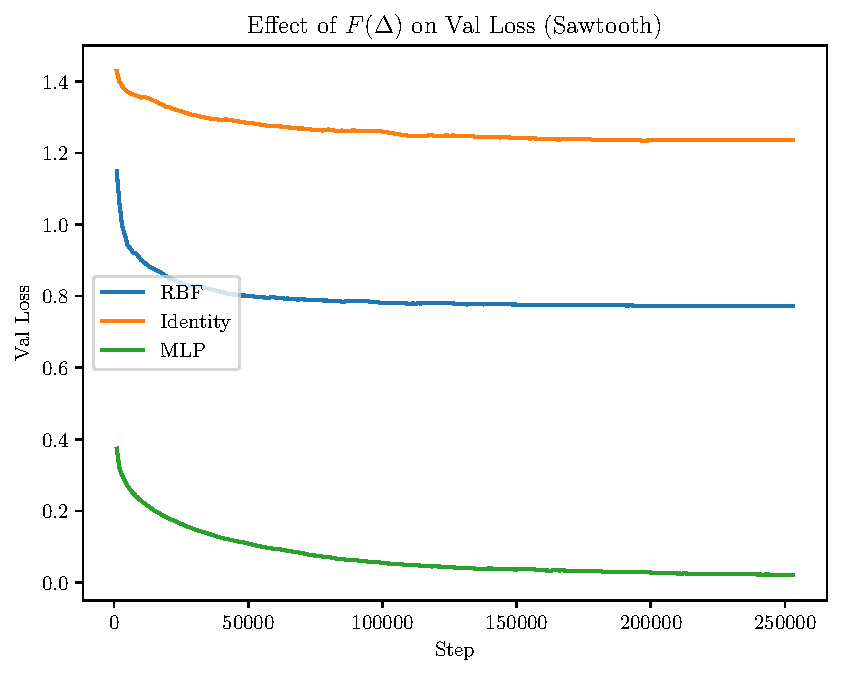
\includegraphics[width=0.6\linewidth]{./F-on-loss.pdf}
	\caption{Relative Attention Functions on Validation Loss for the TETNP on the 1D Sawtooth Dataset. Lower validation loss is better.}
	\label{fig:relative-attn-func-1d}
\end{figure}

\autoref{fig:relative-attn-func-1d} presents the validation loss curves for the TNP with different relative attention functions. The results shows that the MLP function outperforms the other two functions by a large margin. This can be attributed to the MLPs ability to \textbf{learn} representations whilst the other two functions have a fixed closed form. We note that the RBF function performs better than the identity function since the effect of adding the raw difference corrupts the dot product attention. We can conclude that the MLP function is the best function out of three we considered. The computational cost of using the MLP function is not significantly higher than the other two functions, since the MLP is very small.



\section{Optimizing Hyperparameters}

The multi-headed attention mechanism in the Transformer Encoder has three hyperparameters that we will investigate. These are
the token embedding dimension of the data ($D_{em}$), the number of attention heads ($N_h$) and the embedding dimension of the attention heads ($D_h$). We will investigate how changing these hyperparameters affects the performance of the model. To gauge the effect of these hyperparameters, we use a 1 million parameter model and reduce the value of one of the hyperparameters and see the effect on the validation loss. This process is repeated for the other hyperparameters to see which hyperparameters have the most effect on the validation loss. 



\begin{figure}[H]
	\centering
	\subfloat[Token Embedding Dimension]{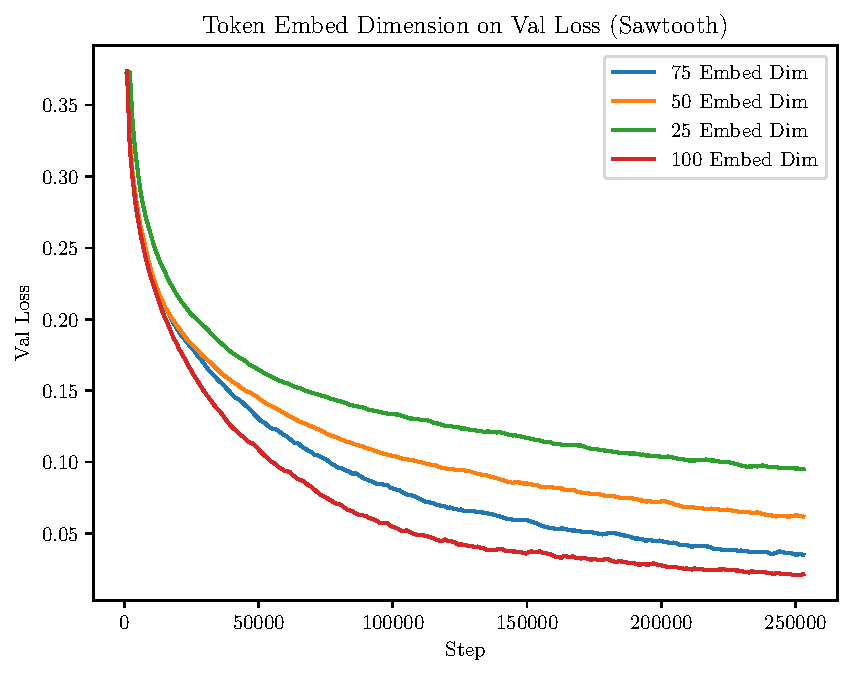
\includegraphics[width=0.5\linewidth]{./embed-dim-on-loss.pdf}\label{fig:hyperparam-optimization-token}}
	\subfloat[Number of Heads]{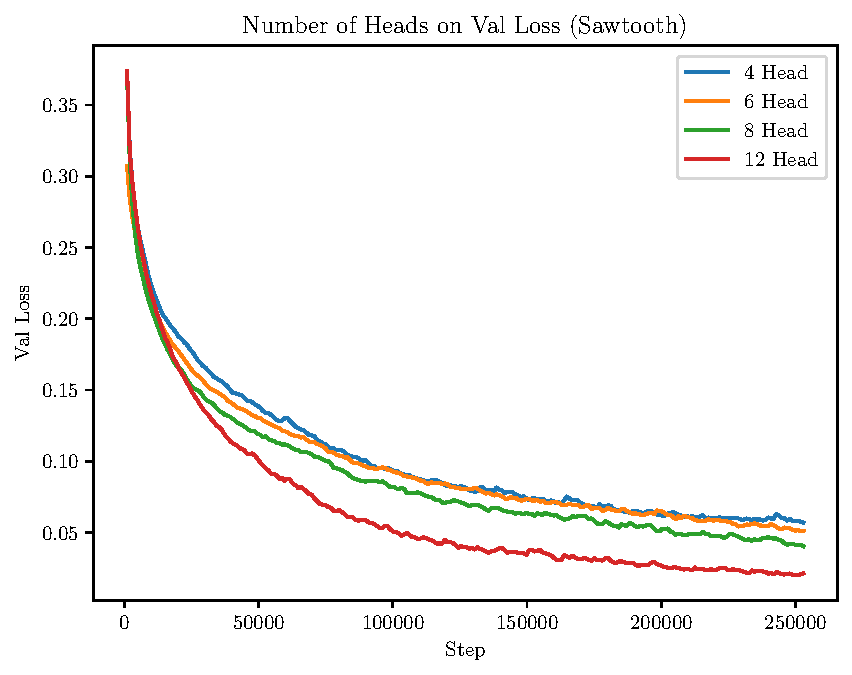
\includegraphics[width=0.5\linewidth]{./head-count-on-loss.pdf}\label{fig:hyperparam-optimization-num}}\\
	\subfloat[Head Embedding Dimension]{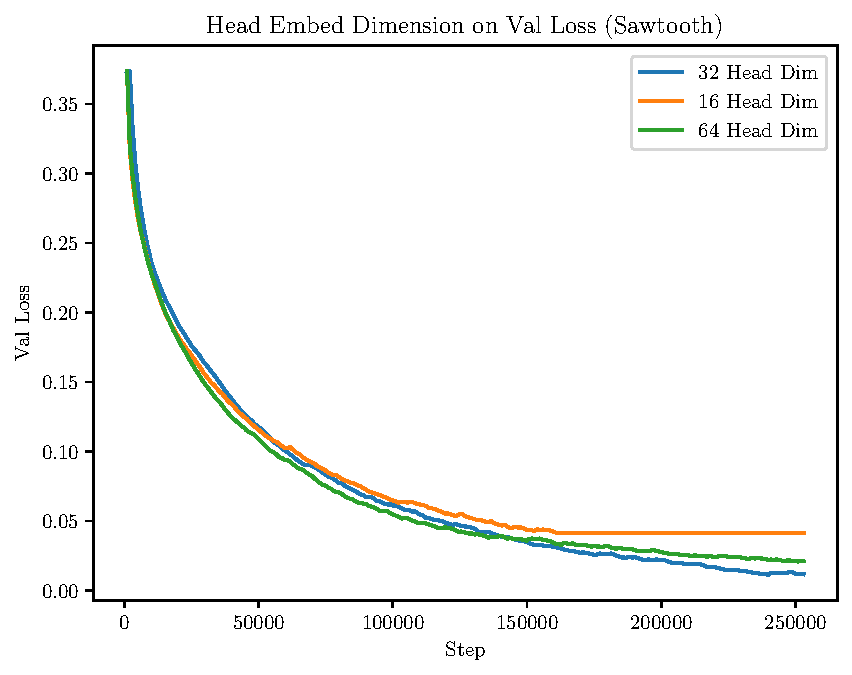
\includegraphics[width=0.5\linewidth]{./head-dim-on-loss.pdf}\label{fig:hyperparam-optimization-head}}
	\caption{Hyperparameter Selection. The three plots consider the effect of reducing the size of a single hyperparameter on the validation loss. Lower validation loss is better.}
	\label{fig:hyperparam-optimization}
\end{figure}

From \autoref{fig:hyperparam-optimization} it is clear that reducing the token embedding dimension has a significant effect on the validation loss, with the number of heads making a smaller difference and the head embedding dimension making very little difference. This highlights the importance of the token embedding dimension when using low dimensional data as the input data (in this case sawtooth function). Furthermore, the head embedding dimension has very little effect on the validation loss, so we can set this to a small value to reduce the number of parameters in the model and distribute the parameters to the other hyperparameters. Using this knowledge, we will now investigate how to select the hyperparameters using a \emph{constant parameter budget} of 1 million parameters. 

% 1m.jpg

\FloatBarrier
\begin{figure}[ht!]
	\centering
	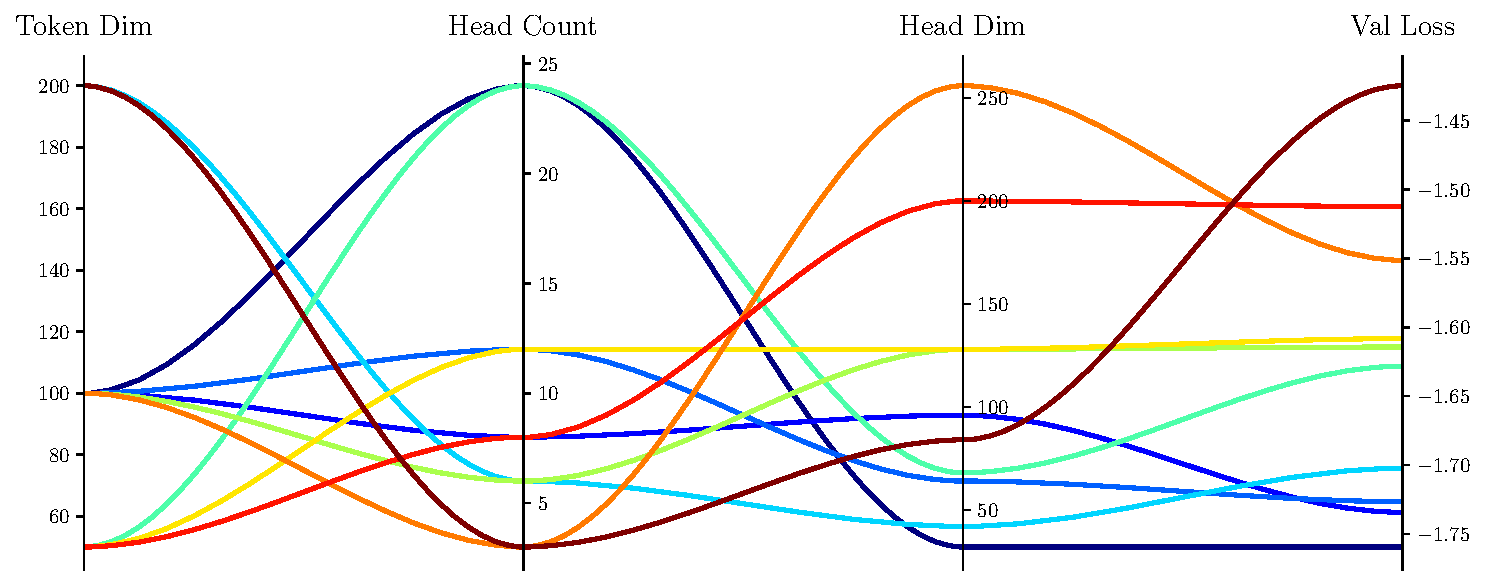
\includegraphics[width=0.9\linewidth]{./model-comparsion-1d.pdf}
	\caption{Constant Parameter Budget Hyperparameter Selection. The parallel coordinates plot shows the validation loss for different hyperparameter configurations. Dark blue is the best and dark red is the worst.}
	\label{fig:1m-parameter-budget}
\end{figure}
\FloatBarrier

\autoref{fig:1m-parameter-budget} shows a parallel coordinates plot of the validation loss for different hyperparameter configurations, where dark blue is the best and dark red is the worst. The model that performs the best has a very high token embedding dimension, high headcount and low head embedding dimension, which is consistent with the previous results. We can also see that if we go too high in the token embedding dimension (200), the model performs worse as we have to sacrifice the number of heads in the transformer. These results give us a set of best practices for selecting hyperparameters for the TNP: \emph{high token embedding dimension, high number of heads and low head embedding dimension}.





\section{TNP vs ConvNP}

% \subsection{Model Fits}

Using the `best' TNP model, we will compare the performance of the ConvNP and TNP on fitting sawtooth and GP (using EQ Kernel) data using 1 million parameters. 

% result.png

\begin{figure}[H]
	\centering
	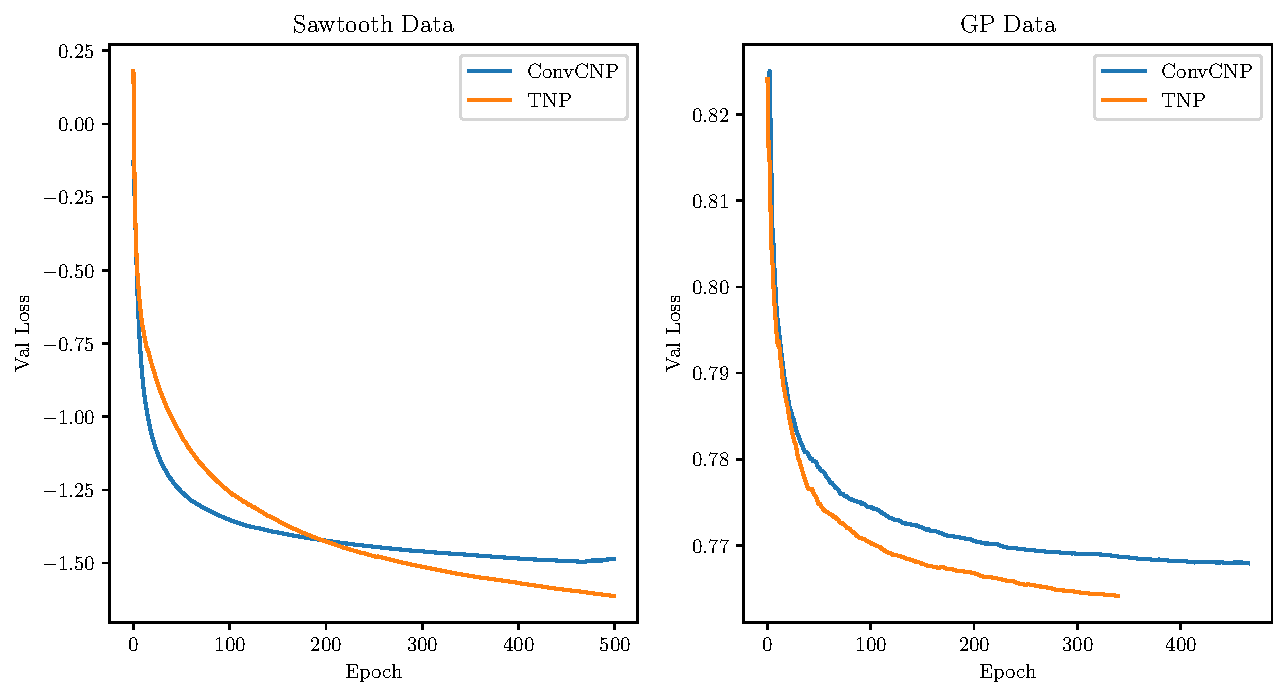
\includegraphics[width=0.5\linewidth]{./convcnp-vs-tetnp-saw-gp.pdf}
	\caption{ConvNP vs TNP on Sawtooth and GP Data}
	\label{fig:conv-tnp-1d-result}
\end{figure}

\autoref{fig:conv-tnp-1d-result} shows the validation loss curves for the ConvNP and TNP on sawtooth and GP data. The validation loss for the TNP is lower than the ConvNP for both datasets which is very promising and indicates the TNP is a better model than the ConvNP. 


\begin{figure}[H]
	\centering
	\subfloat[TNP]{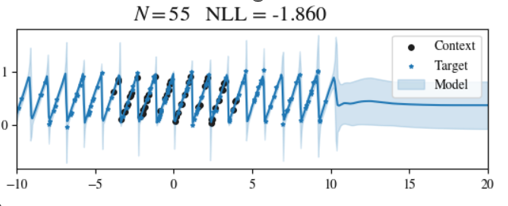
\includegraphics[width=0.47\linewidth]{./tnp_saw.png}\label{fig:1d-sawtooth-comparisons-tnp_saw}}
	\qquad
	\subfloat[ConvNP]{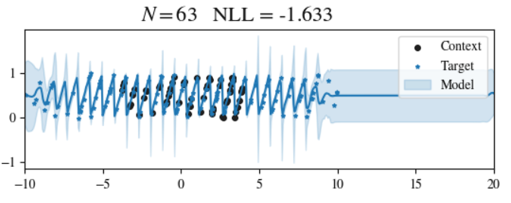
\includegraphics[width=0.47\linewidth]{./convnp_saw.png}\label{fig:1d-sawtooth-comparisons-convnp_saw}}
	\caption{ConvNP vs TNP on Sawtooth Data. The context set inputs are between [-4, 4] and the target set inputs are between [-10, 10] which extends beyond the context set to test the models' extrapolation capabilities.} 
	\label{fig:1d-sawtooth-comparisons}
\end{figure}

Inspecting the model fits on sawtooth data \autoref{fig:1d-sawtooth-comparisons}, we observe that the TNP can extrapolate the structure of the sawtooth function beyond the range of the context set (black points) whilst the ConvNP performs decently but fails to retain the structure as well as the TNP, since the amplitude of the sawtooth reduces the further away from the context set. Hence, we can conclude that the TNP can better understand the structure of the data than the ConvNP.

\subsection{Computational Complexity}

\begin{table}[H]
	\centering
	\begin{tabular}{@{}llccc@{}}
	\toprule
	$N_c$ & $N_t$ & ConvNP  & TNP   & TETNP \\ \midrule
	10    & 10    & 18                 & 13               &  13\\
	100   & 10    & 16                 & 18               &  23\\
	1000  & 10    & 16                 & 339              &  980 \\
	5000  & 10    & 124                & 9357             &  23060\\ \midrule
	10    & 1000  & 36                 & 399              &  25\\
	100   & 1000  & 36                 & 469              &  100\\
	1000  & 1000  & 36                 & 1510             &  1012\\
	5000  & 1000  & 124                & 13480            &  24082\\ \bottomrule
	\end{tabular}
	\caption{Memory Usage in inference of the ConvNP and TETNP on 1D data using $N_c$ context points and $N_t$ target points.}
	\label{tab:memory-usage-comparison}
\end{table}

\autoref{tab:memory-usage-comparison} shows that the TETNP uses drastically more memory than the ConvNP for the same number of context and target points. This is due to the quadratic complexity of the TETNP which scales with $\mathcal{O}(N_c^2 + N_cN_t)$ compared to the linear complexity of the ConvNP which scales with $\mathcal{O}(N_cD_x^3 + N_tD_x)$. Whilst on the 1D dataset the ConvNP is more memory efficient, the TETNPs complexity does not scale with the number of dimensions of the data, whilst the ConvNP \emph{scales cubically with the number of dimensions}. This may suggest that the TETNP is more suitable for high-dimensional data than the ConvNP since the TETNP has a fixed memory cost per dimension. We will investigate this in the next chapter on 2D datasets to see if the discrepancy in memory usage is still present.

\ifSubfilesClassLoaded{%
    \printbibliography{}
}{} 


\end{document}